\documentclass[dvips,dvipdfm,pdftex]{llncs}
\usepackage[utf8]{inputenc}
\usepackage{amsmath}
\usepackage{amsfonts}
\usepackage{amssymb}
\usepackage[dvips,dvipdfm,pdftex]{graphicx}
\usepackage{pgfplotstable}
\usepackage{array}
\usepackage{booktabs}
\usepackage{morefloats}
\usepackage{etex}
\usepackage{listings}
\usepackage{float}

\title{Semi-supervised Hidden Markov Random Fields (HMRF) Kmeans. Theory to Implementation\\}
\author{Dimitrios Pritsos and Efstathios Stamatatos}
\institute{University of the Aegean\\Karlovassi, Samos \textendash{} 83200, Greece.\\\{dpritsos, stamatatos\}@aegean.gr }

\begin{document}

\maketitle

\begin{abstrat}

\end{abstrat}


\section{Introduction}\label{sec:intro}
The objective of the Semi-supervised Clustering is to incorporate in the procedure of clusters discovery or assignment, the prior knowledge about the skeleton of the clusters schema. There are several efforts on Semi-supervised model inference in both Expectation Maximization (EM) clustering based models and in Agglomerating clustering based models. According to \cite{chapelle2006semi_hmrf_kmeans} there three main groups of EM based semi-supervised clustering methods:

\begin{enumerate}
	\item \emph{Constraints-based mehtods} are using the provided supervision for guiding the algorithm towards a data partitioning which is avoiding (but not prevening) the constraints violation.
	\item \emph{Distance-based approaches} in clustering method with a particular distance funciton; the distance function is parametrized and the parameters values are learned to satisfy the constraints.
	\item \emph{Semi-supervised clustering based on Hidden Markov Random Fields} where the constraint-based and distance-based approaches are combined into \emph{a unified probabilistic model}.
\end{enumerate}

In EM clustering based models there have been several efforts where the labeled data where provided in the clustering model in the form of data-labels pairs or in the initialization phase of theclustering model. In this work we present the Hidden Markov Random Fields Model(HMRF) Kmeans, where the prior knowledge about the structure or skeleton of the clusters schema has been embedded into the model in the form of constraints \cite{basu2004probabilistic}. The HMRF Kmeans is a hard-clustering model due to the \emph{hard} assignment of the data point to one of the a-priori fixednumber of clusters. However, the same models can be transformed into a relatively easy soft-clustering model where of each data point only Maximum a-posteriry Probability (MAP) of the point to bea member of each cluster of th final schema.

The HMRF Kmeans Semi-supervised clustering method it has been implemented, in this work, for being tested on the Web Genre Identification (WGI) Information Retrieval (IR) taxonomy problem.Therefore, here we only present the model inference procedure where the distance measure, a.k.a distortion function/measure, is the cosine similarity because in the IR literature is the distortionmeasure where in most cases maximizes performance in problems where the feature space is particularly large, as in this case. In case one would be interested in changing the model to asoft-clustering method then the probability destiny function of the final model should have been chosen to be some properly parametrized Von Mises Fisher distributions.

Since this work is focusing on the implementation of Semi-supervised HMRF-Kmeans in the IR domain framework, it has to be noted that this Semi-supervised model advantage is the interactivelearning setting where this model can be used \cite{chapelle2006semi_hmrf_kmeans}, since the constraints are provided to the model in two different sets the \emph{Must-Link} and\emph{Cannot-Link}. These sets are not necessarily the same in size or complimentary one to the other.

What it follows is the model inference line of thought based on the there resources \cite{basu2004probabilistic,chapelle2006semi_hmrf_kmeans,bishop2006_EM_general_view}.


\section{Model inference}\label{sec:model_inference}
The objective of a semi-supervised model like HMRF Kmeans is to drive the procedure of clustering schema taking into account the prior knowledge we have about the clusters in the form of\emph{must-link} and \emph{cannot-link} constraints. The main difference in the graphical model of a topical EM algorithm is the nodes of the observed labeled data over the hidden, a.k.a latent,variables as depicted in fig.\ref{fig:hmrf_em}, with red colored arrows and gray shaded nodes.

\begin{figure}[h]
	\begin{center}
		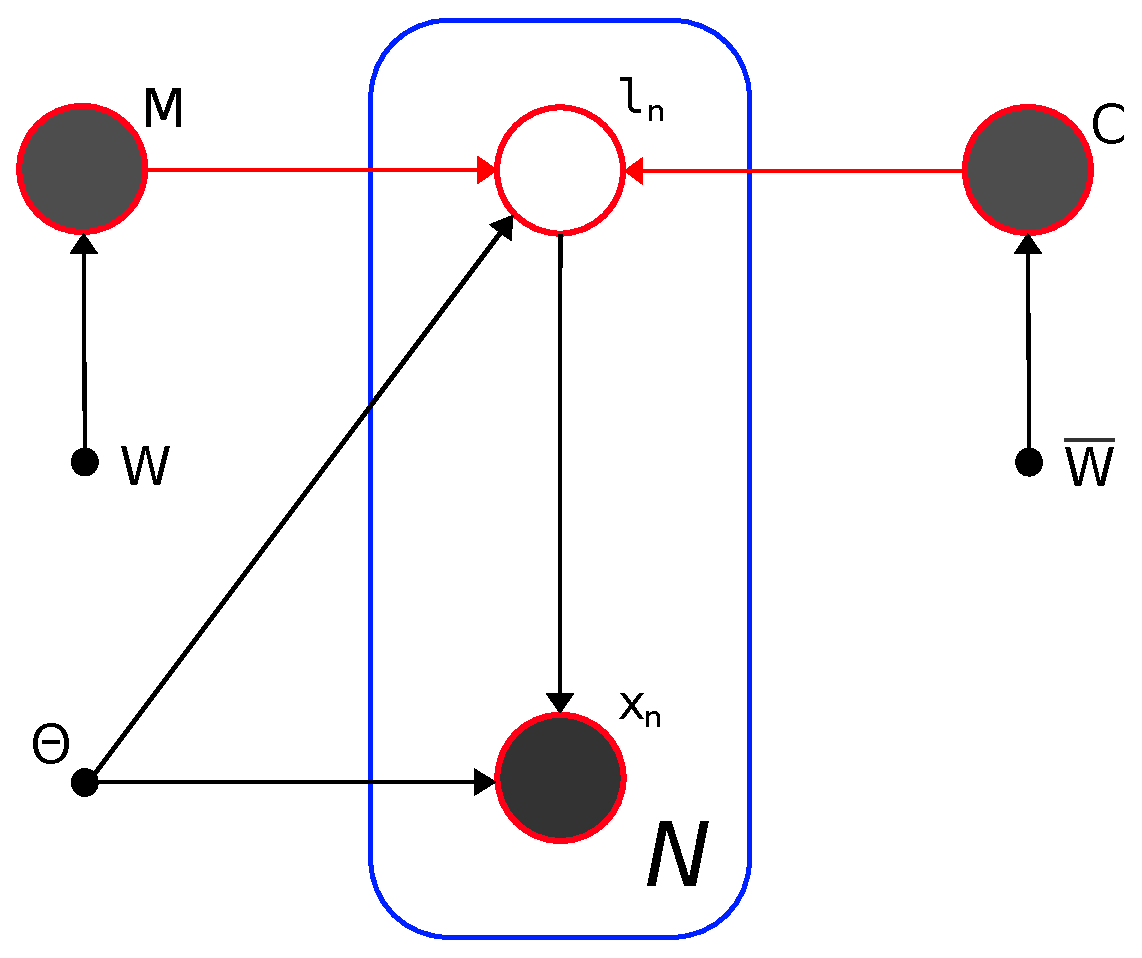
\includegraphics[scale=0.40]{figures/SemiSupervised_HMRF_EM_Graphical_Model.eps}
		\caption{Semi-supervised HMRF Expectation Maximization or Kmeans Clustering Graphical Model.}
		\label{fig:hmrf_em}
	\end{center}
\end{figure}


\bibliographystyle{splncs03}
\bibliography{djumble_doc}

\end{document}
